% 実用性を示すために一連の性能評価を行った。
To show the practicality of the proposed technique, we conducted a series of performance evaluations on our watermarking scheme.
It consisted of three objective evaluations to prove the robustness of the scheme in actual situations, and a user testing to judge that our method can be used without spoiling the listening impression.

% 提案手法の有用性を検証するために、リアルなハードウェア構成でwatermarking schemeの性能評価実験を行った
In these evaluations, we used a prototypical hardware setup assuming real usage.
% ハードウェア構成
% 家庭用ビデオカメラ(型番)とスマートフォン(型番)で構成され、スマートフォンはカメラの外部マイクに固定する
This consisted of a consumer-use digital camcorder (SONY NEX-VG30H) and a smartphone (SAMSUNG Galaxy S) to generate and transmit watermarks.
The phone was attached to the microphone unit of the camera.
% カメラ設定
Movies were recorded in the conventional MPEG-2 format using standard definition image quality, and sound was recorded in 2ch stereo PCM format.
Default values were used for the other configurations of the camcorder.
% スマートフォン設定
Annotation transmitter applications were installed on the smartphone.
The audio output level of the phone was set an appropriate value empirically decided.

\begin{figure}[htbp]
 \begin{center}
  \vspace{5mm}
  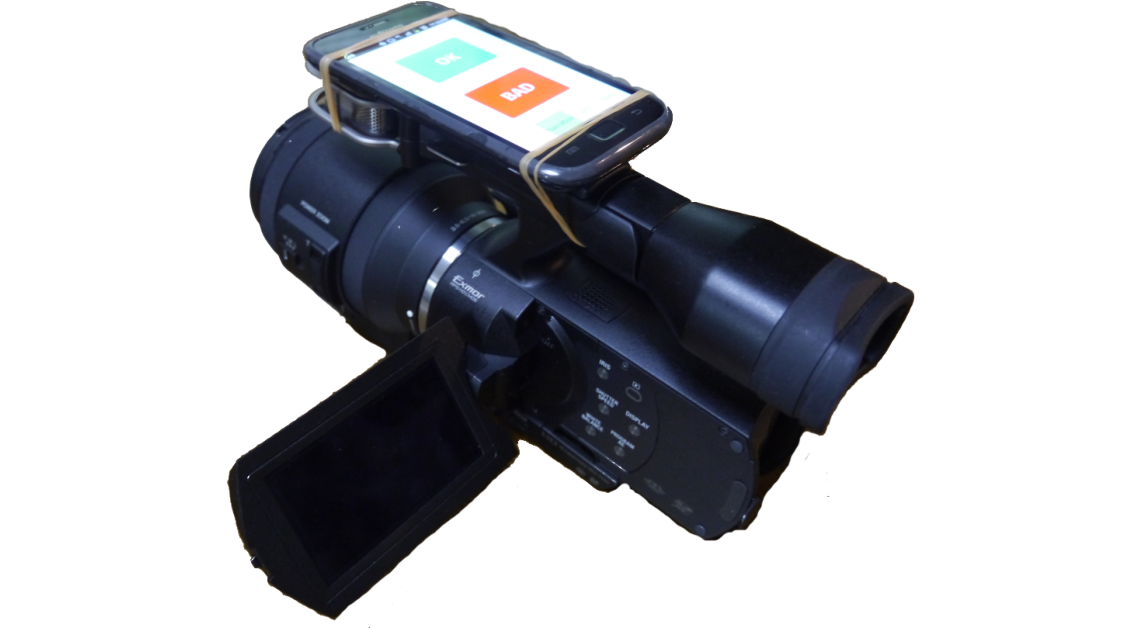
\includegraphics[width=90mm]{evaluation_environment.pdf}
 \end{center}
 \caption{The hardware setup used in the performance evaluations.}
 \label{fig:eval_hard}
\end{figure}
